%%%%%%%%%%%%%%%%%%%%%%%%%%%%%%%%%%%%%%%%%
% Journal Article
% LaTeX Template
% Version 1.3 (9/9/13)
%
% This template has been downloaded from:
% http://www.LaTeXTemplates.com
%
% Original author:
% Frits Wenneker (http://www.howtotex.com)
%
% License:
% CC BY-NC-SA 3.0 (http://creativecommons.org/licenses/by-nc-sa/3.0/)
%
%%%%%%%%%%%%%%%%%%%%%%%%%%%%%%%%%%%%%%%%%

%----------------------------------------------------------------------------------------
%	PACKAGES AND OTHER DOCUMENT CONFIGURATIONS
%----------------------------------------------------------------------------------------

\documentclass[twoside]{article}

\usepackage{lipsum} % Package to generate dummy text throughout this template

\usepackage[sc]{mathpazo} % Use the Palatino font
\usepackage[T1]{fontenc} % Use 8-bit encoding that has 256 glyphs
\linespread{1.05} % Line spacing - Palatino needs more space between lines
\usepackage{microtype} % Slightly tweak font spacing for aesthetics

\usepackage[hmarginratio=1:1,top=32mm,columnsep=20pt]{geometry} % Document margins
\usepackage{multicol} % Used for the two-column layout of the document
\usepackage[hang, small,labelfont=bf,up,textfont=it,up]{caption} % Custom captions under/above floats in tables or figures
\usepackage{booktabs} % Horizontal rules in tables
\usepackage{float} % Required for tables and figures in the multi-column environment - they need to be placed in specific locations with the [H] (e.g. \begin{table}[H])
\usepackage{hyperref} % For hyperlinks in the PDF

\usepackage{lettrine} % The lettrine is the first enlarged letter at the beginning of the text
\usepackage{paralist} % Used for the compactitem environment which makes bullet points with less space between them

\usepackage{abstract} % Allows abstract customization
\renewcommand{\abstractnamefont}{\normalfont\bfseries} % Set the "Abstract" text to bold
\renewcommand{\abstracttextfont}{\normalfont\small\itshape} % Set the abstract itself to small italic text

\usepackage{titlesec} % Allows customization of titles
\renewcommand\thesection{\Roman{section}} % Roman numerals for the sections
\renewcommand\thesubsection{\Roman{subsection}} % Roman numerals for subsections
\titleformat{\section}[block]{\large\scshape\centering}{\thesection.}{1em}{} % Change the look of the section titles
\titleformat{\subsection}[block]{\large}{\thesubsection.}{1em}{} % Change the look of the section titles

\usepackage{fancyhdr} % Headers and footers
\pagestyle{fancy} % All pages have headers and footers
\fancyhead{} % Blank out the default header
\fancyfoot{} % Blank out the default footer
\fancyhead[C]{Effects of Oil Spill on Plant Growth $\bullet$ December 2015} % Custom header text
\fancyfoot[RO,LE]{\thepage} % Custom footer text

\usepackage{graphicx}
\graphicspath{{images/}}

\newcommand{\mean}[1]{\bar{#1}}

%----------------------------------------------------------------------------------------
%	TITLE SECTION
%----------------------------------------------------------------------------------------

\title{\vspace{-15mm}\fontsize{24pt}{10pt}\selectfont\textbf{Effects of Oil Spill on Plant Growth}} % Article title

\author{
\large
\textsc{Derek Elliott}\\[2mm] % Your name
\normalsize University of West Florida \\ % Your institution
\normalsize STA 5176 Statistics Modeling
\date{}
\vspace{-5mm}
}

%----------------------------------------------------------------------------------------

\begin{document}

\maketitle % Insert title

\thispagestyle{fancy} % All pages have headers and footers

%----------------------------------------------------------------------------------------
%	ABSTRACT
%----------------------------------------------------------------------------------------

\begin{abstract}
 
\noindent To test the effectiveness of their cleanup effort after a large oil spill, a study was performed on 80 equal tracts of land, 40 of which were randomly selected from uncontaminated areas, and 40 from the affected areas. The density of \textit{Distichlis spicata} was taken at each site and recorded.  The mean density and variation were found for both groups and it was found that the densities differed by an amount between 5.5 and 17.6 with 95\% confidence.

\end{abstract}

%----------------------------------------------------------------------------------------
%	ARTICLE CONTENTS
%----------------------------------------------------------------------------------------

\begin{multicols}{2} % Two-column layout throughout the main article text

\section{Introduction}

\lettrine[nindent=0em,lines=3]{O}n January 7, 1992 an oil pipeline burst in San Patricio County, Texas and contaminated a marsh near the Chiltipin Creek.  During the process of cleaning the spill, the marsh was burnt and replanted with local fauna.  A year after the burning and replanting, the oil company wanted to evaluate the effectiveness of their effort.  In order to do this the company randomly chose 40 tracts of land that were affected by the spill, and 40 that were not.  The tracts were as similar as possible.  The density of \textit{Distichlis spicata} was to be evaluated to measure the effectiveness.
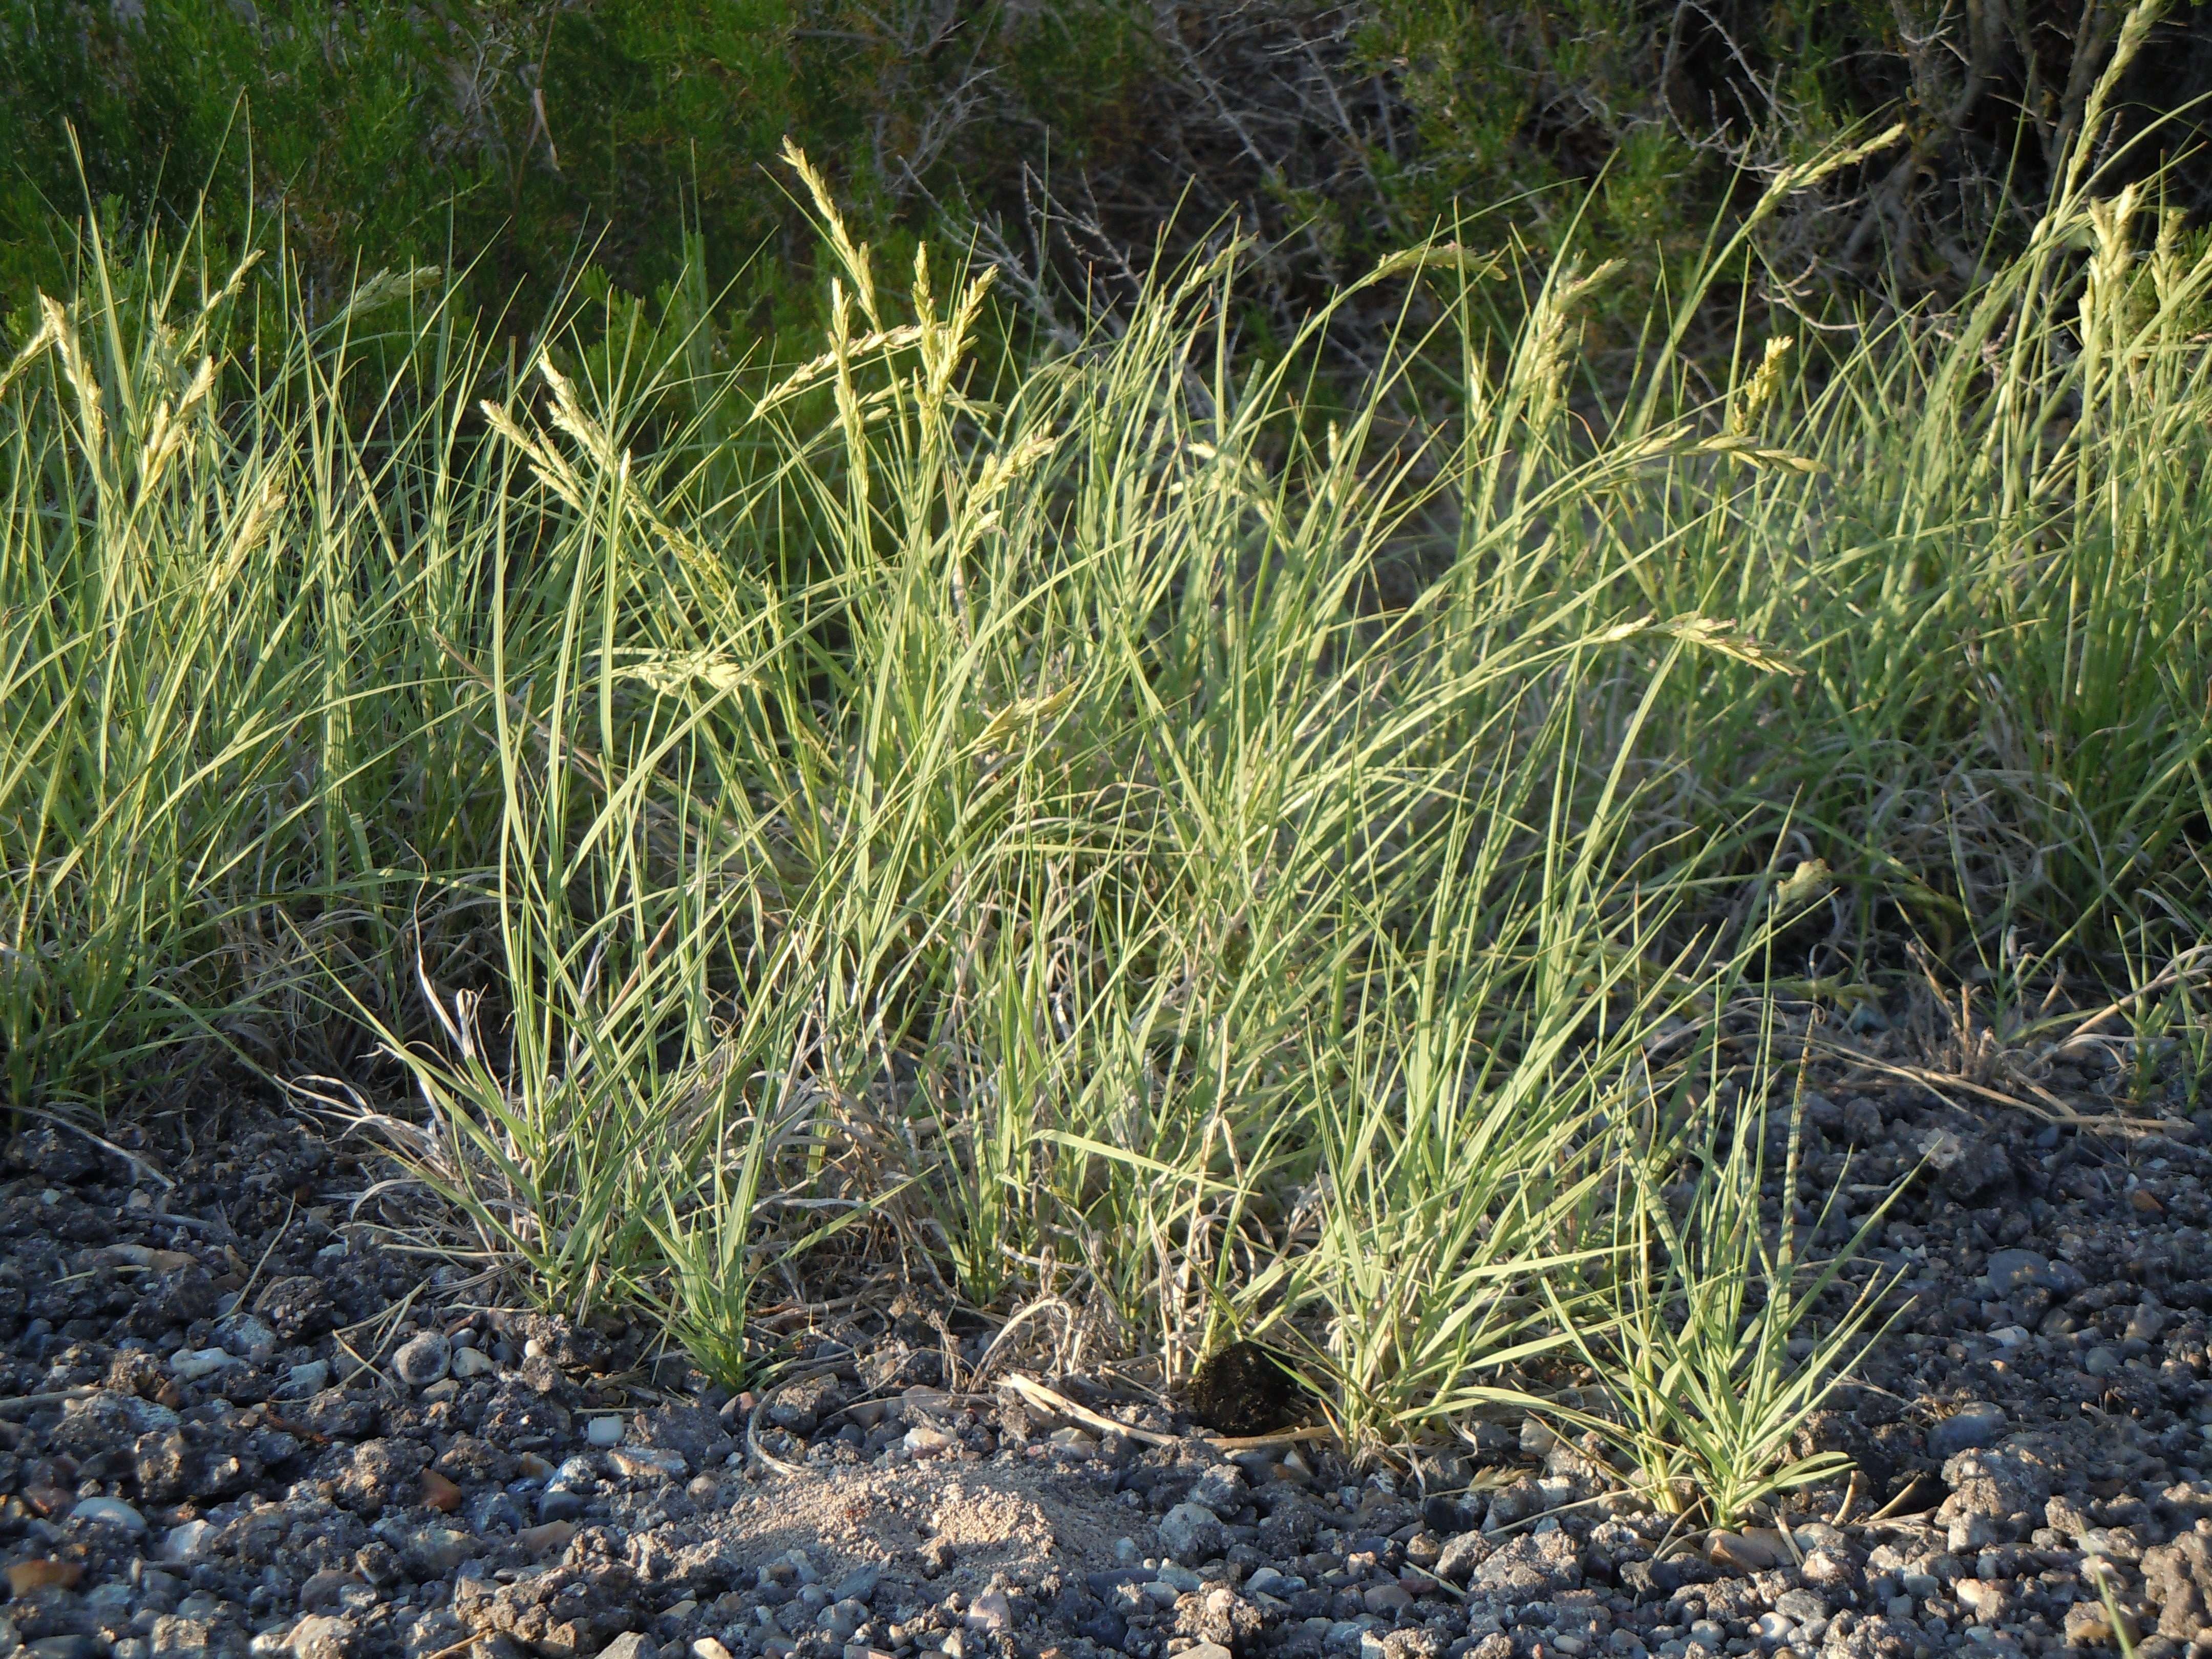
\includegraphics[scale=0.05]{Distichlis_spicata}
\captionof{figure}{Distichlis spicata}

%------------------------------------------------

\section{Data and Methodology}
Based on the boxplot and normal probability graphs, it can be shown that the contaminated sites can be considered normally distributed, but the control sites can not.  Because of this, we can use the two population t test under the hypothesis: $$H_0: \mu_{con} = \mu_{oil}\quad vs. \quad H_I: \mu_{con}>\mu_{oil}$$.


\begin{table}[H]
	\caption{Summary Statistics}
	\centering
	\begin{tabular}{lr|lr}
		\toprule
		\multicolumn{2}{c}{Control Tracts} & \multicolumn{2}{c}{Contaminated Tracts} \\
		\midrule
		Mean: & $38.48$ & Mean: & $26.93$ \\
		Median: & $41.5$ & Median & $26.00$ \\
		St. Dev: & $16.37$ & St. Dev & $9.88$ \\
		n: & $40$ & n: & $40$ \\
		\bottomrule
	\end{tabular}
\end{table}

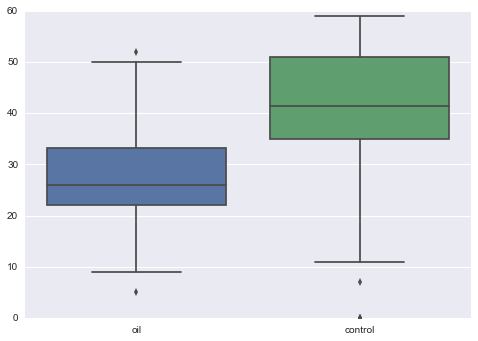
\includegraphics[scale=0.35]{output_5_1}
\captionof{figure}{Box Plot of Contaminated and Control Sites}

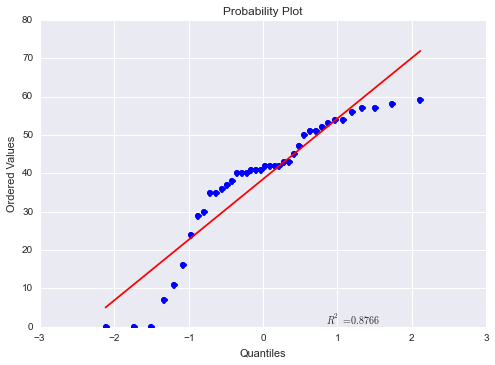
\includegraphics[scale=0.35]{output_7_0}
\captionof{figure}{Normal Probability Plot of Control Sites.}

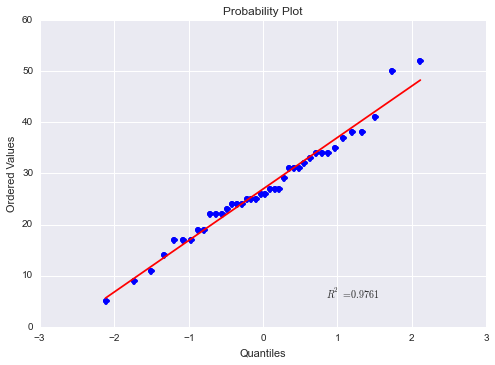
\includegraphics[scale=0.35]{output_6_0}
\captionof{figure}{Normal Probability Plot of Contaminated Sites}

%------------------------------------------------

\section{Analysis of Data}

Because we are using the two population t test, the test statistic is: $$t = \frac{\mean{x}-\mean{y}}{\sqrt{\frac{S_{con}}{n_{1}}+\frac{S_{oil}}{n_{2}}}}$$ Where $\mean{x}$, $\mean{y}$, $S_{con}^2$, and $S_{oil}^2$ are given in Table 1.  This gives $t = 3.82$.  Given the hypothesis above, in order to reject $H_0$, it must be shown that $t>t_{\alpha, dof}$.  To do this, the degrees of freedom must be computed using the following formula: $$dof = \frac{(n_{con}-1)(n_{oil}-1)}{(1-c)^2(n_{con}-1)+c^2(n_{oil}-1)}$$ Where c is given by $$c = \frac{\frac{S_{con}^2}{n_{con}}}{\sqrt{\frac{S_{con}^2}{n_{con}} + \frac{S_{oil}^2}{n_{oil}}}}$$  This gives $dof = 64$.  Then, from tables, $t_{0.05, 64} = 1.699$.  Thus, $t = 3.82 > t_{0.05, 64} = 1.699$ and $H_0$ can be rejected.  Then, the 95\% confidence interval for $\mu_{con} - \mu_{oil}$ is given by: $$(\mu_{con} - \mu_{oil}) = t_{\alpha/2, dof}\sqrt{\frac{S_{con}^2}{n_{con}} + \frac{S_{oil}^2}{n_{oil}}}$$  Thus, the 95\% confidence interval for $\mu_{con} - \mu_{oil}$ is $11.55 \pm 6.05$.

%------------------------------------------------

\section{Concluding Remarks}
Based on the results in the previous section, it is known that the density of \textit{Distichlis spicata} is statistically higher in uncontaminated tracts than it is in contaminated tracts, by an amount between $5.05$ and $17.6$.  Further, these results would need to be given back to the environmental scientists who would need to evaluate them and come to a conclusion as to whether the areas that were affected by the oil spill have satisfactorily returned to pre-spill conditions.

%----------------------------------------------------------------------------------------
%	REFERENCE LIST
%----------------------------------------------------------------------------------------

\begin{thebibliography}{99} % Bibliography - this is intentionally simple in this template

\bibitem[Ott and Longnecker, 2010]{Figueredo:2009dg}
Ott, R.~Lyman. and Longnecker, Michael. (2010).
\newblock \textit{An Introduction to Statistical Methods and Data Analysis}, 325--330.
 
\end{thebibliography}

%----------------------------------------------------------------------------------------

\end{multicols}

\end{document}
